\chapter{Introduction}
\label{cap:intro}

Human history presents a series of important inventions that resulted in great advances to society. From the seemingly simple ones, such as the cart wheel, going through steam power, up to the transistor, most of the narrative is focused on the economic or social consequences of these inventions. The path that led from the scientific discoveries to the inventions, many of those being considered as the foundations of modern society, is, most of the time, not mentioned, perhaps because the application was straightforward or in some cases, the discovery was made by chance. The discovery of penicillin is one of the most famous of these cases \cite{Flemming1929}. 

Of course, in other cases the path was already set by theory, and what people today describe as an invention was the realization, in a controllable and predictable way, of one or more phenomena that were completely or partially understood at the time. The internal combustion engine and the steam-powered engine may be seen, from that point of view, as the biggest proofs of the success of thermodynamic theory, as well as the Bose-Einstein Condensates, which might enable quantum computing in the future \cite{Vinit2013}.

The pressure of society for solutions to many problems is another ingredient in this process, and lately the economic aspect of that pressure is the most obvious one. The semiconductor industry exemplifies that really well via Moore's law \cite{Moore1998}, which states that the number of transistors that can be built on top of a single integrated circuit roughly doubles each year. The reasons are not mainly due to technical advances, but mostly related to the cost of production. It is ironic that now we might have reached a limit for that law, due to the fact that devices cannot shrink beyond atomic sizes.

From the point of view of theory-driven inventions, one of the most interesting and promising ones is the case of the memristor. This new electronic device was proposed theoretically nearly 40 years ago \cite{Chua1971,Chua1976} but its realization was only claimed in 2008 \cite{Williams2008}. That realization brought many promises of a complete revolution in the computer business, but so far the device has not been completely understood, hence, its application is still not possible.

\section{Memristor: the missing circuit element}

In 1971, Leon O. Chua, using a symmetry argument, proposes the existence of a fourth fundamental circuit element, which he names the memristor \cite{Chua1971}. This new device would complete the set given by the known elements---resistor, capacitor, and inductor---in an elegant way: while the resistance may be interpreted as a quantity defining the relation between voltage $v$ and current $i$, the capacitor for the relation between charge $q$ and voltage $v$, and the inductor for the connection between magnetic flux $\varphi$ and current $i$, and taking into account the definition of current $(i=\nicefrac{dq}{dt})$ and Faraday's law $(v=\nicefrac{d\varphi}{dt})$, there would still be a missing relation: the one between the magnetic flux and charge. This relation is, thus, the definition of the memristor. The complete picture of these relations is shown on figure \ref{fig:circuit-elements}.

This new device is characterized by its memristance $M$, and the relation between the voltage and the current through the device was given by
\begin{equation}
  v(t) = M[q(t)]i(t),
  \label{eq:v_x_i_memristor}
\end{equation}
where the dependency of $M$ on $q$ can be easily shown if one uses the definition of current and Faraday's law on the relation between the magnetic flux and the charge\footnote{$v(t)=\frac{d \varphi}{d t} = \frac{d f}{d q} \frac{d q}{d t} = M[q(t)]i(t)$. Note that the explicit dependence on $q$ is only possible if the relation is not linear on $q$.} 
\begin{equation}
  \varphi=f(q).
  \label{eq:phi_x_q} 
\end{equation}

\begin{center}
  \begin{figure}[h!]
      \begin{center}
        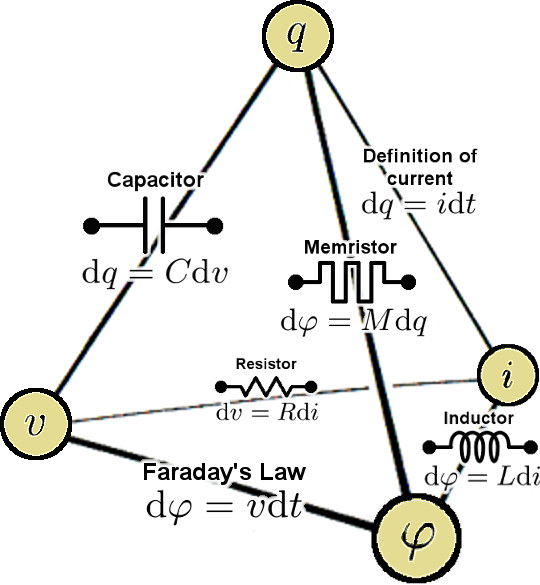
\includegraphics[width=0.5\textwidth]{img/memristor-vars.jpg}
        %\includegraphics[width=0.4\textwidth]{img/circuit-elements.jpg}
      \end{center}
      \caption{The four circuit elements and all relations between the fundamental circuit variables (charge $q$, voltage $v$, current $i$, and magnetic flux $\varphi$). At the edge that connects $q$ and $\varphi$ the symbol propoed by Chua for the memristor is depicted.}%At the bottom right square the symbol proposed by Chua for the memristor is depicted \cite{Williams2008}}.
      \label{fig:circuit-elements} 
  \end{figure}
\end{center}

According to Chua, the relation given by \ref{eq:v_x_i_memristor}, indicates that the memristance will depend on the amount of charge going through the device in a given time, {\em i. e.} this quantity will {\em remember} how much charge has passed by, and thus, the name memristor was proposed. Two examples of $i \times V$ curves obtained via equation \ref{eq:v_x_i_memristor} for different non-linear forms of equation \ref{eq:phi_x_q} are presented in Figure \ref{fig:lissajous-theo}. From those figures it is possible to extract two fundamental properties of Chua's memristor: i) the curves always cross themselves at the origin, meaning that no energy is stored in this device due to lack of delay between $i$ and $v$---usually referred to as {\em the pinched hysteresis loop} shape of the $i \times V$ curve---, and ii) that there are two possible slopes for the $i \times V$ curves at the origin, {\em i. e.} two values of electrical resistance.
\begin{center}
  \begin{figure}[h!]
    \begin{center}
      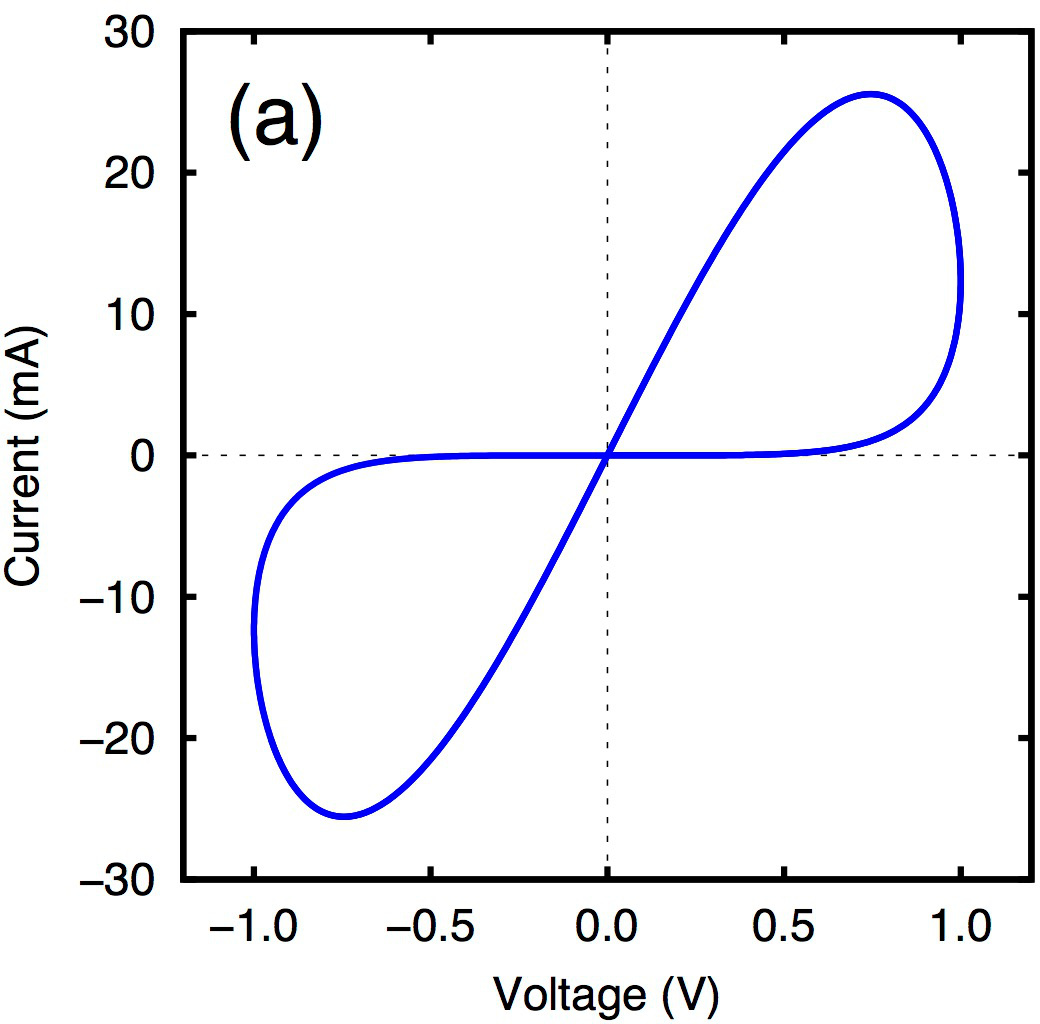
\includegraphics[height=6cm]{img/lissajous-01.jpg}
      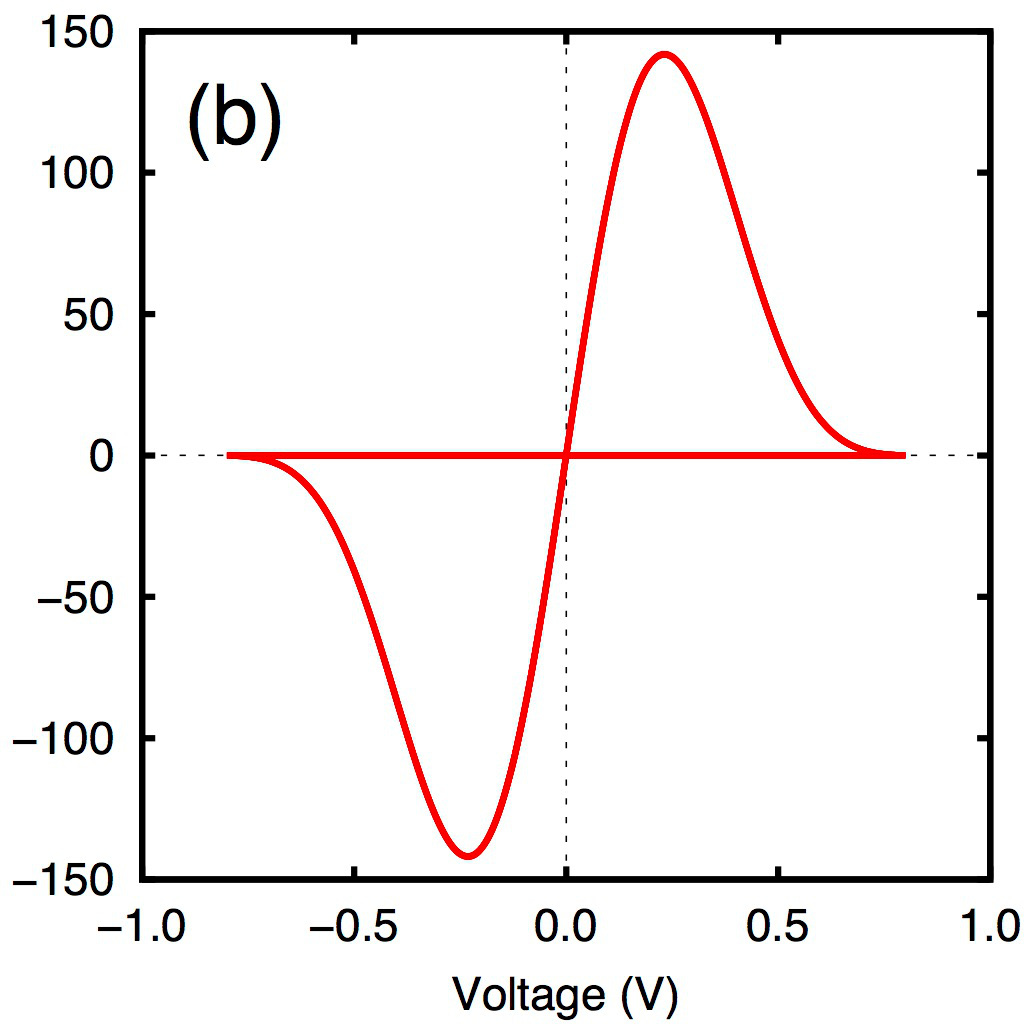
\includegraphics[height=6cm]{img/lissajous-02.jpg}
      \caption{Examples of $i \times V$ curves for (a) a third-order polynomial dependence of $\varphi$ on $q$ and (b) an exponential dependence.} 
      \label{fig:lissajous-theo} 
    \end{center}
  \end{figure}
\end{center}

A few years later, in 1976, Chua and Kang expanded the concept of memristor to a class of memristive systems \cite{Chua1976}. According to them, these devices are described by a set of equations,
\begin{align}
 v(t)&=R(x,i,t)i(t)\label{eq:memristive_devices_res} \\
 \frac{dx}{dt}&=f(x,i,t) \label{eq:memristive_devices_var}
\end{align}
where $x$ is a $n$-dimensional state vector which condensates all possible parameters that describe the state of the device, $f$ is a $n$-dimensional vector function and $R$ is a scalar continuous function. Explicit time-dependence is not mandatory for those quantities. In the particular case of the memristor, we have $x = q$, \(R(x,i,t) = M(q)\), and \(f(x,i,t) = \nicefrac{dq}{dt} = i\).

These two papers remained fairly unnoticed by the scientific community, and, until recently, this interesting theory was lacking its realization. Even though memory effects on thin films were reported throughout the 1970's, 80's, 90's and even at the beginning of the century \cite{Dearnaley1970,Pinto1971,Oxley1977,Hirose1976,Beck2000,Upadhyaya1995,Kim2006}, the connection of these results with Chua's theory was not noticed. This scenario was completely changed when an experimental group claimed they found the first memristor.

\section{The Missing Memristor Found}

In 2008, an experimental group led by Staley Williams at HP labs, working on resistance switching on thin films of titanium dioxide (TiO$_2$) claims the realization of Chua's memristor \cite{Williams2008}. A sketch of the device and the corresponding $i \times V$ curve obtained in their experiment is presented on figures \ref{fig:curva_hp_labs} (a) and (b). This realization of the memristor, as well as the following devices, is a two-terminal system where two metallic electrodes are separated by an active layer composed of a semiconductor or instulator thin film. Its $i \times V$ curve is such that both properties of memristor can be noticed: the crossing at the origin and the distinct low-bias resistances.
\begin{center}
  \begin{figure}[h!]
    \begin{center}
    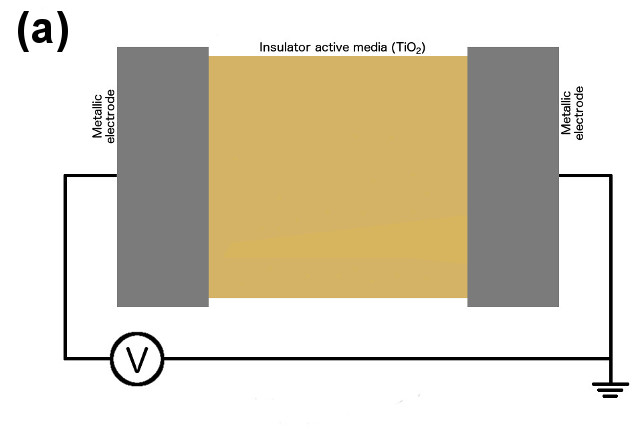
\includegraphics[height=6.2cm]{img/memristor-intro.jpg}
    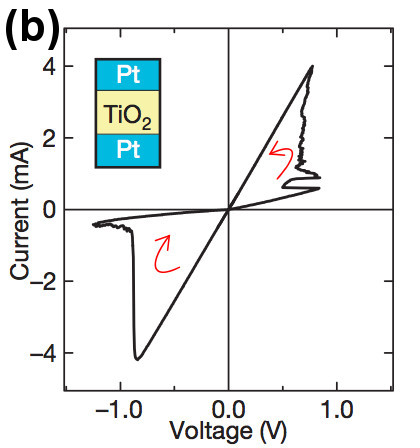
\includegraphics[height=6.2cm]{img/exp-HP.jpg}
      %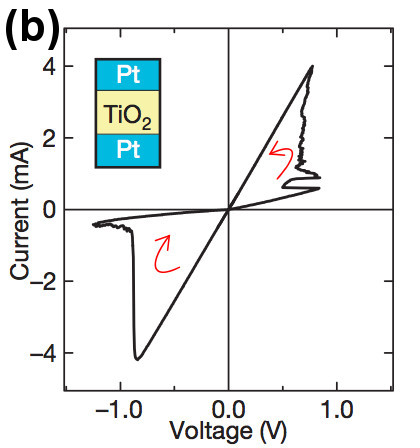
\includegraphics[width=0.7\textwidth]{img/exp-HP.jpg}
      \caption{(a) Schematic view of the TiO$_2$-based memristor. The voltage is applied at the opposing metallic electrodes throught the active layer. (b)Experimental $i \times V$ curve of a TiO$_2$-based memristor. The inset depicts the Metal/Insulator/Metal structure of the device\cite{Williams2008}.} 
      \label{fig:curva_hp_labs} 
    \end{center}
  \end{figure}
\end{center}

The model proposed by the authors considers the thin film as two one-dimensional resistors ($\mathcal{R}_{ON}$ and $\mathcal{R}_{OFF}$) connected in series and weighted by the width $w$ of the doped layer (the dopant being positively charged oxygen vacancies) of the semiconductor,
\begin{equation}
 v(t)=\left[\mathcal{R}_{ON}\frac{w(t)}{D}+\mathcal{R}_{OFF}\left(1-\frac{w(t)}{D}\right)\right]i(t),
 \label{eq:ohmic_hp_labs}
\end{equation}
where $D$ is the width of the thin film and consequently the upper boundary for $w$ ($0 \leq w \leq D$). The time evolution of $w$, {\em i. e.} the dynamics of the extent of the doped and undoped parts, is given by a phenomenological drift-diffusion model $\nicefrac{dw}{dt}= \mu_V E = \mu_V\left(\nicefrac{\mathcal{R}_{ON}}{D}\right)i(t)$, where $\mu_V$ is the dopant mobility and $E$ is the electric field, assumed constant across the device. Integration of this equation and substitution into equation \ref{eq:ohmic_hp_labs}, considering \(\mathcal{R}_{ON} \ll \mathcal{R}_{OFF}\), leads to
\begin{equation}
  v(t) = \mathcal{R}_{OFF}\left[1-\mu_V\frac{\mathcal{R}_{ON}}{D^2}q(t)\right]i(t)=M[q(t)]i(t).
  \label{eq:memristance_hp_labs}
\end{equation}

Due to the explicit dependence on $q(t)$ in \ref{eq:memristance_hp_labs}, this device is considered as the first realization of Chua's memristor. The explanation provided by the authors for the fact that nobody had never seen the realization of a memristor before was that people were not looking at the right scale: while the resistor, capacitor and inductor are feasible at the microscopic scale, the memristive property would be perceived only at the nanoscale ($D \sim 10^{-9}$ m). However, a recent historical review on memristors show that this might not be the case: gas-discharge tubes, tungsten filaments, high-pressure mercury-vapour lamps, among other macroscopic materials where a physical property presents inertia were reported to have the same characteristic $i \times V$ curves \cite{Prodromakis2012}.

As the time span between Chua's theoretical memristor and the experimental realization was nearly 40 years, the case of the memristor can be considered as a particular one: when although the theory was known, the realization was not at all simple.
\newpage

\section{Memristors and switching devices}

There was a sudden interest of the scientific community on the memristor after the paper from William's group in 2008. It happened not only because it was the first time one showed the equivalence between the memristor and the already known electric resistance switching devices, but also because the memristor brought a big promise for the computer memory industry. Those devices would be faster, denser, and less power-consuming than memory devices available today, mainly due to their smaller sizes and 3D stacking possibility (see reference \cite{Jeong2012} for a detailed comparison between memory technologies). 

In fact, the resistance switching property was already being investigated for quite some time, even before Chua's first paper on memristors. In 1965 Chopra obtains $i \times V$ curves for a series of oxides (Nb, Ta, and Ti) thin films sandwiched between metallic electrodes and detected a negative resistance when a threshold current was reached \cite{Chopra1965}. In 1968 Johnson observes unusual changes in TiO$_2$-rutile crystals' electrical resistance, which he attributed to the presence of H$^+$ impurities \cite{Johnson1968}. A recent historical compilation \cite{Prodromakis2012} shows that memristive phenomena have been detected for the last two centuries, even before the discovery of the other electronic devices such as the resistor, capacitor, and inductor. Many authors report unexpected behaviors for the electrical resistance of oxides, from the early 60's until quite recently before the William's group claim \cite{Hickmott1962,Argall1968,Oxley1977,Hirose1976,Upadhyaya1995,Beck2000,Waser2007}, but none of them could point out the link between their results and Chua's theory. There is even a model, older than Chua's, for resistance switching, given in a 1967 paper by Simmons and Verderber \cite{Simmons1967} where they study resistance switching in silicon oxide thin films containing gold impurities, but it has drawn very little attention. This lack of interest can be understood from the technological scenario of that time, where silicon integrated circuits were becoming the work horse of the computer industry and remained undisputed until the end of the 90's, when people realized that Moore's law \cite{Moore1998} could not be sustained in the long run.

Of course, not all feedback is positive to William's group paper. A few authors questioned whether the realization of the memristor was actually a discovery or just a claim looking for huge impact and consequently huge profits. Among those, we can identify some interesting arguing whether the memristor and the resistance switching devices are the same thing or not \cite{Gale2014}. One of the main points against William's group claim and the equivalence between memristors and switching devices is that while the first is defined by Chua's theory from electromagnetic theory---and the crucial point is that it explicitly includes magnetism in its mathematical derivation---, the switching devices proposed mechanisms, so far, do not rely on that. Leon Chua himself has given his opinion recently, stating that "Resistance switching memories are memristors" \cite{Chua2011} and "If it's pinched it's a memristor" \cite{Chua2014}. His point is that the required properties for a device to be considered a memristor are given by its $i \times V$ curve characteristics---a pinched hysteresis shape is the memristor's fingerprint---, which are fullfiled by the switching devices. He even presents a general differential equation to define the state vector (as defined by equation \ref{eq:memristive_devices_var}) of a memristor in terms of power series,
\begin{equation}
  \frac{dx}{dt} = \sum_{i=1}^m a_i x^i + \sum_{j=1}^n b_j i^j + \sum_{j,k=1}^{p,r} c_{jk} x^j i^k
  \label{eq:chua_2011}
\end{equation}
where the careful choice of the parameters \(\{a_i, b_i, c_{ij}\}\) would be enough to fit any experimental $i \times V$ curve of a memristor. For instance, the HP memristor model is described by \(x = w(t)\) and \(a_i = c_{ij} = 0\), \(b_1 = \mu_V \left(\nicefrac{\mathcal{R}_{ON}}{D}\right)\), and \(b_i = 0\) for \(i>1\). Despite the discussion between supporters and deniers of the equivalence between these devices, many authors today use both terms interchangeably \cite{Yang2012,Waser2009,Szot2011,Strachan2009}, which means that the first group is the larger one. I adopt the same position in this thesis, thus, from this point on the names {\em memristor} and {\em resistance switching device} or just {\em switching device} will be used indistinctly to refer to the same system. 

In a general way, memristors are composed of a thin insulator film---usually referred to as the active media---sandwiched between two electrodes. Some of the materials used as active media are binary oxides (TiO$_2$ \cite{Choi2005,Hickmott1962,Argall1968,Kim2013c,Yang2011,Miao2011b,Williams2008}, Ta$_2$O$_5$ \cite{Pinto1971,Hickmott1962,Miao2011a,Beck2000}, TaO$_x$ \cite{Yang2010,Miao2012}, Nb$_2$O$_5$ \cite{Pinto1971,Kundozerova2012}, NiO \cite{Seo2004,Wang2013}, ZnO \cite{Huang2013,Chen2013}, SiO \cite{Simmons1967,Hickmott1962,Chang2013}, Al$_2$O$_3$ \cite{Hickmott1962}, ZrO$_2$ \cite{Hickmott1962,Kim2013b}, HfO$_2$ \cite{Syu2013,Luo2013}, Fe$_2$O$_3$ \cite{Kim2013a}, and WO$_3$ \cite{He2013}), perovskites (PbTiO$_3$ \cite{Pilch2014}, SrTiO$_3$ \cite{Muenstermann2010,Szot2006}, SrZrO$_3$ \cite{Beck2000,Rossel2001,Guo2013}, (Pr,Ca)MnO$_3$ \cite{Ignatiev2006}, (Sm,Ca)MnO$_3$/(La,Sr)MnO$_3$ \cite{Sawa2006}), silicon \cite{Dong2008,Mehonic2012}, and other systems as sulfides (Ag$_2$S$_3$ \cite{Hirose1976}, (Zn,Cd)S \cite{VanderSluis2003}), carbon-based systems (C$_{60}$, C$_{70}$, and C$_{84}$ encapsulated inside double-walled carbon nanotubes \cite{Li2009}), and polymers (poly-spirofluorene \cite{Gomes2008}). Electrode materials comprise a wide range of metals as Au \cite{Chopra1965,Hickmott1962,Beck2000}, Ag \cite{Chopra1965}, Al \cite{Chopra1965,Choi2005,Hickmott1962}, Pt \cite{Kim2013b,Choi2005,Miao2011a,Beck2000,Yang2010,Miao2012,Huang2013,Chen2013}, Ru \cite{Choi2005}, Ta \cite{Hickmott1962,Miao2011a,Yang2010,Miao2012}, Zr \cite{Hickmott1962}, Ti \cite{Hickmott1962,Syu2013}, Cu \cite{Waser2009}, TiN \cite{Kim2013b,Syu2013}, and many other materials (see ref. \cite{Pan2014} and references therein). A key point that binds all these materials in the large group of memristive materials is that for all cases defects are present in the materials, either in the form of point defects in a crystalline system, or by use of amorphous thin films.

\begin{center}
  \begin{figure}[h!]
    \begin{center}

      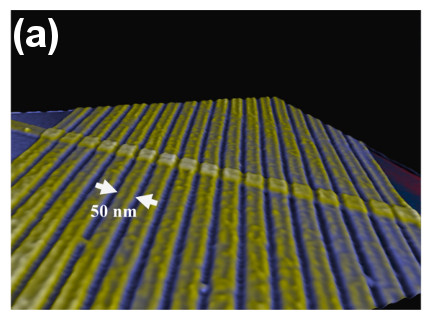
\includegraphics[height=5.5cm]{img/MiaoNanotechnology2011.jpg}
      %\includegraphics[height=5.5cm]{img/memristor.jpg}
      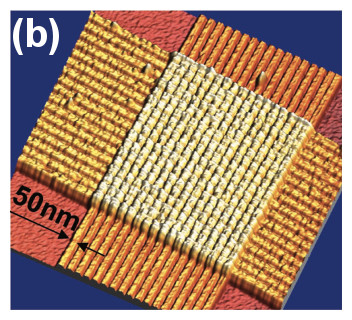
\includegraphics[height=5.5cm]{img/MiaoAdvMat2011.jpg}
      %\includegraphics[height=3.6cm]{img/YangAPL2012.jpg}
      \caption{Atomic force microscopy image of a crossbar junction network of (a) TaO-based \cite{Miao2011a} and (b) TiO$_2$-based memristors \cite{Miao2011b}.} 
      \label{fig:sketch-mem} 
    \end{center}
  \end{figure}
\end{center}

The memristor's two-terminal device spatial arrangement is obtained using lithography for the metallic layers and many deposition methods for the active layer, as sputtering \cite{Miao2011b}, pulsed laser deposition \cite{Muenstermann2010}, low-pressure chemical vapor deposition \cite{Chang2013}, and by oxidation of the bottom electrode \cite{Jeong2012}. One important detail is that none of those techniques yield perfect crystals: defects are always present. For high-density memories, the memristor cells are structured in a crossbar junction network, as shown in Figures \ref{fig:sketch-mem} (a) and (b), where each electrode crossing enclosures a memristor.

\begin{center}
  \begin{figure}[h!]
    \begin{center}
      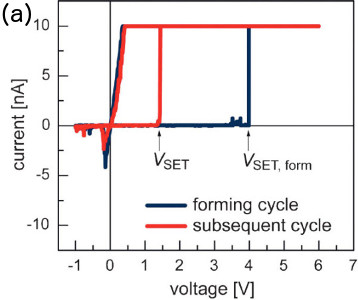
\includegraphics[height=4.1cm]{img/Wasser2009-electroform.jpg}
      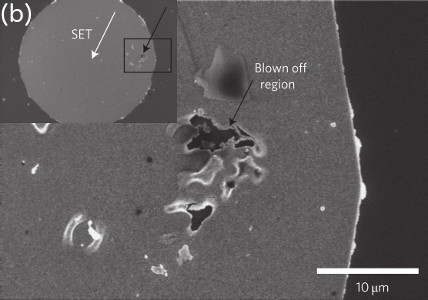
\includegraphics[height=4.1cm]{img/Kwon2010NatureNanoBolhas.jpg}
      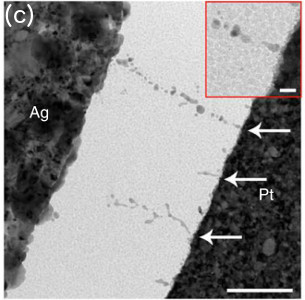
\includegraphics[height=4.1cm]{img/Yang2012NatureCommCanais.jpg}
      \caption{(a) $i \times V$ curve for a Cu/SiO$_2$/Pt memristor where the forming cycle and subsequent cycles are depicted \cite{Waser2009}. The constant current of 10 nA is the compliance current. (b) Scanning Electron Microscope (SEM) image of the blown-off region of top-electrode of a Pt/TiO$_2$/Pt device \cite{Miao2011a}. This result is explained by the formation of O$_2$ under this electrode after the electroforming. (c) Ag channels formed after electroforming step on top of a planar Ag/SiO$_2$/Pt device \cite{Yang2012}. Scale bar is 200 nm.} 
      \label{fig:electroform-channel} 
    \end{center}
  \end{figure}
\end{center}

After the process of structurally building the device, an electroforming step is required for the majority of the reported systems to properly switch. This process consists of a soft breakdown of the dielectric, which is performed by subjecting the pristine device to a voltage larger than usual switching voltage, keeping the resulting current bounded by the so-called compliance current (see fig. \ref{fig:electroform-channel}). At a microscopic level, it is believed to result in local heating and filamentary conduction before structural changes take place in the active media due to ionic migration \cite{Sharma2014,Yalon2012}. The main consequence of such process is the introduction of defects in the active media, such as oxygen vacancies---evidenced by the escape of O$_2$ gas from oxides \cite{Kwon2010,Jeong2012,Chen2013,Miao2011a}---or metal impurities---usually due to ionic migration of Cu$^+$ and Ag$^+$ species from the electrodes into the active media \cite{Yang2012,Yang2014,Guo2007}. Experimental data for both cases is presented in figure \ref{fig:electroform-channel}.

The devices after electroforming can store information via its switcheable resistance state. In order to write information, a voltage beyond a threshold value is required and this process can take place in two modes: unipolar or bipolar. In the unipolar mode, the switching from a high-resistance state (HRS) to a low-resistance state (LRS) (usually referred to as the reset process) and the other way around (the set process) can be performed using the same polarity of the applied voltage. On the other hand, devices operating in the bipolar regime are set and reset using different polarities. These two modes of operation are illustrated in figure \ref{fig:unipolar-bipolar}. The read operation is performed using a small bias, such that the system is not disturbed from its current resistance state.

Current devices show a great promise for future memory technologies. Switching times as fast as picoseconds and $\mathcal{R}_{ON}/\mathcal{R}_{OFF}$ ratios higher than 10$^9$ have been reported \cite{Pan2014}. Another important feature is the number of read/write cycles a device can stand, which is usually referred to as the endurance. For TaO-based devices, up to 10$^9$ reliable cycles have been reported \cite{Yang2010}. Due to the fact that once the system is set or reset the lifetime of programmed state is stable for years \cite{Lee2011,Waser2007}, the memristor also presents the potential to unify the volatile (such as random access memories - RAM) and non-volatile memories (magnetic media, flash). This new device shows the best attributes of the latter, as fast switching times and low power consumption, and of the former, as long retention times and large number of read/write cycles. For a comparison with other technologies such as RAM and flash, a comprehensive review is presented by Jeong {\em et al.} \cite{Jeong2012} as well as others \cite{Fujisaki2010, Chua2011, Kim2011, Waser2007, Waser2009, Yang2012, Szot2011, Pan2014}.

\begin{center}
  \begin{figure}[h!]
    \begin{center}
      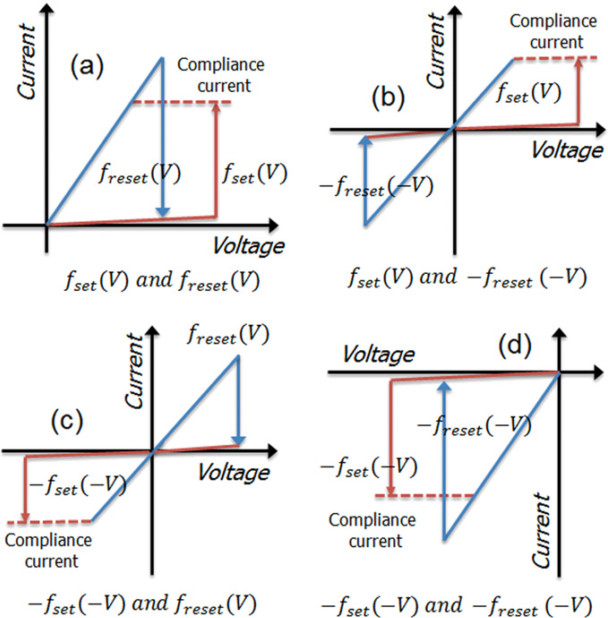
\includegraphics[height=11cm]{img/Jeong2012RepProgPhys.jpg}
      \caption{Schematic $i \times V$ curves for memristors. In (a) and (d) one sees unipolar switching while in (b) and (c) the bipolar regime is shown. $f_{\text{set}}$ and $f_{\text{reset}}$ are the sections of the $i \times V$ curves related to each process \cite{Jeong2012}.}
      \label{fig:unipolar-bipolar} 
    \end{center}
  \end{figure}
\end{center}

Even though the memristor presents remarkable properties for next-generation memory technologies, its immediate application is hindered by the lack of understanding of the working principle at a microscopic scale. For example, the switching time presents a strong non-linear dependency with respect to the applied voltage, which in turn leads to statistical variation of that time \cite{Medeiros-Ribeiro2011,Pickett2009}, making it very difficult to efficiently operate the device in a controlled fashion. Another important point is that the memristive property arises in a wide range of systems, thus suggesting that either the working principle is not material-related or it has a variety of diferent origins.
\newpage

\section{Models}
\label{sec:models}

Given the current scenario, many models were proposed to explain these promising devices, and two of them could be considered the best accepted so far: ionic drift-diffusion and purely electronic models. As explained earlier, the electroforming process is responsible for introducing a number of defects inside the active layer, which in turn may acquire the shape of a channel, as shown in Figures \ref{fig:electroform-channel} (c) and \ref{fig:canais-TiO}. The ionic model states that these channels will short circuit the device (span the whole device width, connecting both electrodes) while in the ON state, and a small part of that channel will be removed increasing the resistance of the device into the OFF state once the polarity is reversed or due to Joule heating in the unipolar case \cite{Pickett2009}. The fast switching times are made compatible with this model by assuming that the diffusion barriers for ions inside the active material can be lowered by presence of large electric fields and/or high temperature spots. This picture is known in the literature as the field/temperature enhanced acceleration of ionic movement \cite{Ielmini2012,Ielmini2011}.
\begin{center}
  \begin{figure}[h!]
    \begin{center}
      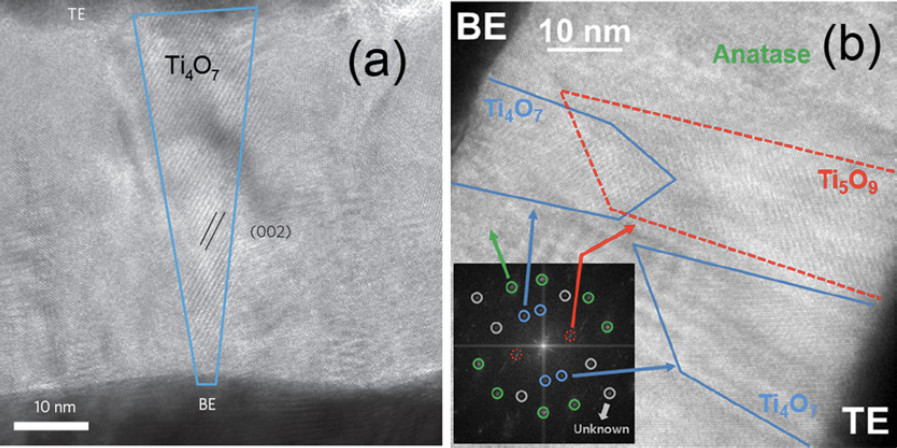
\includegraphics[width=12cm]{img/Jeong2012canaisTiO.jpg}
      \caption{Transmission Electron Microscope (TEM) images of (a) single Ti$_4$O$_7$ channel \cite{Kwon2010} and (b) multiple Ti$_4$O$_7$ and Ti$_5$O$_9$ channels \cite{HwanKim2011} inside TiO-based memristors. The inset in (b) shows X-ray diffraction data used to characterize the different parts of the active region.} 
      \label{fig:canais-TiO} 
    \end{center}
  \end{figure}
\end{center}

On the other hand, purely electronic models, which can be tracked down to the late 60's, explain the switching phenomena mainly according to the trapping and de-trapping of charges inside the active region due to the presence of intrinsic or extrinsic impurities \cite{Simmons1967}. Other less popular electronic models claim that the switching is caused by metal/insulator Mott transitions \cite{Stoliar2013,Yalishev2012} or modulation of the Schottky barrier \cite{Marchewka2015}. In any of those cases, there is an apparent dilemma from the energetic point of view: if the LHR and HRS are electronic by nature, there may be a potential barrier that separate those states. Such barrier should be low enough that the switching time is fast but in order for the final states to be stable, the same barrier should be high. This picture is referred to as the "voltage-time dilemma" by Schroeder {\em et al.} \cite{Schroeder2010}. The main issue in this work is that the authors assume a solution to the Poisson equation and give an {\em ansatz} solution as the potential energy barrier for electrons injected into the active media ({\em i. e.} the conduction band minimum - CBM) but do not solve it. As I will show, it is possible to overcome the voltage-time dilemma by performing a self-consistent calculation that treats the problem in a more realistic fashion.

Summarizing, even though many experimental results point out the existence of filaments inside the active region of the devices, there is no direct proof of the filament formation and subsequent dissolution within the timescale reported for the switching process. The electronic models however, were not throught explored, and theoretical and/or computational studies are scarce. An atomic scale picture of the memristor is still missing, even though it is a consensus that the understanding of the processes taking place at this scale is the key to unravel the memristor. Questions as why the device switches so fast and at the same time stores information for such a long time, or how unipolar switchin works, or even why the memristive property is observed in so many materials that, in principle, present no simmilarities at all, are still waiting for definite answers.

\section{The contribution of this work}
\label{sec:contrib}

Our contribution is to understand the memristor from a theoretical point of view. As most of the data on memristors was obtained experimentally---and thus via indirect measurements---, it is currently very difficult to understand the processes taking place inside the devices during switching. Even the properties of the nanometric structures formed inside the devices are not completely known. In this scenario, density functional theory (DFT) calculations are already proven to be a viable and powerfull tool able to probe the atomic-level interactions within a nanoscale system. The fast developement of numerical algorithms and hardware, as well as of the theory itself, has enabled the spread of many DFT-based electronic structure codes in the last two decades \cite{Becke2014,Capelle2006}.

The choice of focusing on TiO$_2$-based devices is twofold: i) it is one of the most popular materials for devices manufacturing \cite{Szot2011,Gale2014,Jeong2012,Miao2011b}, as is the case of the prototypical device developed by HP \cite{Williams2008}, and ii) the intrinsic defects, oxygen vacancies and titanium interstitials are known to present stable charge states \cite{Janotti2010,Lee2012} within the bandgap. Within ion-drift models, this last feature is considered only due to the action of the electric field on charged vacancies \cite{Strukov2009,Williams2008,Kwon2010}, but no recent reports on the changes of the properties of these materials upon charging and de-charging are available.

One of the first steps in any study is to choose one or more methodologies out of many. As it is known in the electronic structure community, DFT is based on an approximation for the exchange and correlation contributions to the total energy of the system \cite{Capelle2006,Becke2014}. The ground state total energy of a quantum system composed by $n$ interacting electrons subject to an external potential is a functional of the ground state electronic density within this theory. There are many levels of approximation that can be used and several ways to express this functional dependecy, the key difference is how the \textit{exchange} and \textit{correlation functionals}\footnote{From now on we will refer to the \textit{exchange} and \textit{correlation functionals} used simply as \textit{functionals}} are written given a degree of the approximation. The accuracy and suitability of the different functionals when used for specific systems should always be probed in these kinds of studies. With that in mind, our first work was to compare three different functionals: the local density approximation (LDA) \cite{Ceperley1980}, the generalized-gradient-approach (GGA) functional proposed by Perdew, Burke and Ernzerhof (PBE) \cite{Perdew1997} parametrized for better description of solids and surfaces (PBESol) \cite{Perdew2008}, the same functional with the on-site Hubbard $U$ parameter for $d$ electrons \cite{Dudarev1998} and the screened hybrid functional by Heyd, Scuseria and Ernzerhof (HSE) \cite{Heyd2003}. This study was performed for TiO$_2$ and its oxygen-deficient phases known as the Mangéli phases---present inside the TiO-based memristors after electroforming---and is presented in chapter \ref{chap:raw}.

The next question that naturally arose was how the oxygen-deficient phases interact electronically with the surrounding TiO$_2$ matrix. To answer that question, the band offset between TiO$_2$-rutile and the Magnéli phase Ti$_4$O$_7$ was obtained and is presented in chapter \ref{chap:band-offset}. To achieve this goal, a supercell approach was employed, and using crystallographic operations the Magnéli structure was derived from the rutile one, making it possible to match the structures without any stress on the interface.

Another key point was the stability of the oxygen-deficient phases. Some studies already pointed out that the Magnéli phases are more stable than the rutile structure containing some ammount of defects---either oxygen vacancies or titanium insterstitials---that mimics their non-stoichiometric composition \cite{Liborio2008}, but the exchange of electrons with the electrodes was not taken into account. We performed thermodynamical calculations to asses the stability of Ti$_2$O$_3$, Ti$_4$O$_7$, and Ti$_5$O$_9$ in such situation. Our results, reported in chapter \ref{chap:charges}, indicated that these systems could in principle store positive charges in a similar way to what happens when point defects are present inside insulators or semiconductors. This charging and de-charging process could change the electronic transport mechanism in those systems and thus enable electronic switching.

The last part of this work was to solve the Poisson equation for the memristors. This was performed using the code developed in collaboration with Dr. Hannes Raebiger from Yokohama National University, while he was working as a visiting professor at UFABC. The numerical results shown in chapter \ref{chap:bandbend} pointed out the possibility of an electronic mechanism for switching, based on deffect-assisted charge trapping inside the active media. Multiple solutions of the Poisson equation were interpreted as diferent resistance states, as each one reveals the true profile of the barrier for incoming electrons in memristors. 

%The contribution of this work is to understand the memristor from a theoretical point of view. Using density functional theory (DFT) calculations for TiO$_2$---one of the most popular materials used to build memristors---and its oxygen-deficient phases known as the Mangéli phases---present inside the TiO-based memristors after electroforming---, we could understand the properties of those materials at atomic level and evaluate their energy band alignment at the interfaces. The stability of the Magnéli phases was studied from the point of view of thermodynamic total-energy calculations when the system is allowed to exchange atoms and electrons with reservoirs. The role of charging and de-charging of electron traps was elucidated and numerical solutions of the Poisson equation were obtained, revealing the true profile of the barrier for electrons in memristors. 